\documentclass{exam}
\usepackage{amssymb}
\pagestyle{headandfoot}
\firstpageheadrule
\runningheadrule
\firstpageheader{CT - Topic 4}{}{Sam Robbins}
\runningheader{CT - Topic 4}{What type of problem do we have to solve?}{Sam Robbins}
\firstpagefooter{}{}{}
\runningfooter{}{}{}

\renewcommand{\solutiontitle}{\noindent\textbf{Solution:}\par\noindent}

\printanswers
\usepackage{graphicx}
\marksnotpoints
\bracketedpoints
\pointsdroppedatright
\pointsinrightmargin
\begin{document}
\begin{center}
	\underline{\huge What type of problem do we have to solve?}
\end{center}
\begin{questions}

\question[3]Give three different notions relating to general problem solving that are key concerns in Computer Science?
\begin{solution}[2in]
	\begin{itemize}
		\item Computation
		\item Resource
		\item Correctness
	\end{itemize}
\end{solution}

\question[4]What is abstraction in relation to real-world problem solving? How does abstraction in Computer Science differ from abstraction in other subjects? 
\begin{solution}[2in]
	\begin{itemize}
		\item Hiding information, such as to make the problem easier to solve
		\item In Computer Science, abstraction is concerned with information hiding, whereas in other subjects abstraction is more concerned with information neglect
	\end{itemize}
\end{solution}

\question[5]What is the real-world travelling salesman problem? Explain how this problem is usually abstracted so that it is amenable to computational solution. Illustrate how this abstraction might not be in keeping with reality.
\begin{solution}[2in]
\begin{itemize}
	\item Computing the shortest tour of a given collection of cities so as to same a resource of interest
	\item If just shortest distance is required, then it could be abstracted to the cities and the distances between them
	\item If time was important, then distributions that model traffic conditions rather than distances would need to be created for each pair of cities
	\item This might not be in keeping with reality because the distribution for traffic is a complicated one and may not be modelled correctly.
\end{itemize}
\end{solution}
\newpage
\question[7]What is the real-world map-colouring problem? Explain how we might abstract this problem as a graph colouring problem. What is a planar graph? Explain how planar graphs and maps are related. Is every graph a planar graph?
\begin{solution}[2in]
\begin{itemize}
	\item Given a plane map of regions, each contained within a continuous border, can you colour the regions of the map with 3 colours so that if any two regions touch they must be coloured differently?
	\item This can be abstracted into a graph, as all the important information is just if two regions touch
	\item \textbf{Planar Graph} - A graph that can be drawn in a plane without any graph edges crossing
	\item Every map can be turned into a planar graph
	\item Not every graph is a planar graph, some will have edges that cross
\end{itemize}
\end{solution}

\question[4]What is the real-world scheduling problem? Explain how we might abstract this problem as a graph colouring problem.
\begin{solution}[2in]
\begin{itemize}
	\item You have a set of jobs that need to be allocated to t (equal length) time slots. Jobs can be scheduled in any time slot, but some pairs of jobs are in conflict as they cannot be scheduled in the same time slot. Can we decide whether there is a schedule for the jobs so that the number of time slots is at most t?
	\item Jobs are abstracted as vertices, and two vertices are joined by an edge if the corresponding jobs are in conflict
	\item There is a schedule of the jobs in t slots so that no conflicting jobs occupy the same slot if, and only if, the corresponding graph can be coloured using t colours
\end{itemize}
\end{solution}
\newpage
\question[4]What is the real-world register allocation problem? Explain how we might abstract this problem as a graph colouring problem.
\begin{solution}[2in]
\begin{itemize}
	\item A large number of program variables are allocated to a small number (k) of CPU registers
	\item Not all program variables are in use at the same time
	\item If two program variables are in use at the same time, then they have to be assigned to different registers
	\item Can we decide whether every program variable can be assigned to one of our k registers so that if two program variables are in use at the same time then they are necessarily assigned to different registers
	\item Program variables are abstracted as vertices, two vertices are joined by an edge if the corresponding program variables are in use at the same time
	\item There is an allocation of program variables to k registers so that if any two program variables are in use at the same time then they have to be allocated different registers if, and only if, the corresponding graph can be coloured using k colours.
\end{itemize}
\end{solution}

\question[4]What is the real-world frequency assignment problem? Explain how we might abstract this problem as a graph colouring problem.
\begin{solution}[2in]
	\begin{itemize}
		\item Consider a network of radio transmitters, each of which must be assigned one of f operating frequencies
		\item If two nearby transmitters are operating on the same frequency then they have the potential to interfere with each other, the frequencies assigned to such pairs of transmitters are required to be distinct
		\item Can we decide whether we can allocate a frequency, from a set of f frequencies, to every transmitter, so that any pair of nearby transmitters mist have different frequencies
		\item Transmitters are abstracted as vertices, and two vertices are joined by an edge if the corresponding transmitters are nearby each other.
		\item There is an assignment of f frequencies to transmitters if, and only if, the corresponding graph can be coloured using f colours
	\end{itemize}
\end{solution}


\question[2]What is the essential rule to bear in mind when developing an abstraction	of a real-world problem?
\begin{solution}[2in]
	The abstractions mirror reality sufficiently closely so that any conclusions reached remain valid as regards the real world problem
\end{solution}
\newpage
\question[2]Give a precise definition of a decision problem.
\begin{solution}[2in]
	A decision problem D consists of:
	\begin{itemize}
		\item a set of instances I
		\item A subset $Y\subseteq I$ of yes instances
	\end{itemize}
\end{solution}

\question[20]What is a graph? What is a proper colouring of a graph and an optimal
colouring of a graph? Describe two different algorithms (in English)
that enable you to colour graphs. Explain whether or not your
algorithms yield an optimal colouring (you may use graphs to illustrate
your answer if you wish). Show how your algorithms proceed when you
wish to decide whether the graph in Fig. 1 can be coloured using 4
colours
	\begin{center}
	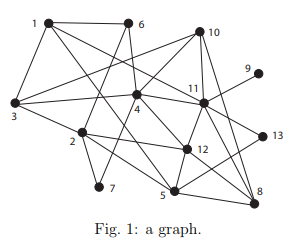
\includegraphics[scale=0.7]{graph}
\end{center}
\begin{solution}[2in]
A graph, G=(V,E), has a finite set V of vertices and a set E of pairs of
distinct vertices where no edge is repeated and (in an undirected
graph) (u,v)=(v,u). A proper colouring is a colouring in which any two
adjacent vertices are coloured differently, the optimal colouring is a
proper colouring that uses the smallest number of colours.\\
\\
Algorithm one: work through the nodes in increasing order and
colour using the smallest available colour. This will always yield a
proper colouring, but may not yield an optimal colouring, however if
it does yield an optimal colouring, that colouring is correct.\\
\\
Algorithm two: chose a node that can be coloured using the lowest
colour possible, if there are multiple nodes that can be coloured with
that colour, then chose the node with the lowest vertex order. Once no
other nodes can be coloured using that colour, move onto the next
colour.\\
\\
Both algorithms produce an identical 3-colouring for the graph.\\
\\
1:1, 2:1,3:2,4:1,5:2,6:2,7:2,8:1,9:1,10:3,11:2,12:3,13:1
\end{solution}
\newpage
\question[2]What is the famous Four Colour Theorem in graph theory?
\begin{solution}[2in]
	Every planar graph can be properly coloured using just 4 colours
\end{solution}

\question[2]Give a (not necessarily precise) definition of what it means for an algorithm to be greedy.
\begin{solution}[2in]
	An algorithm that works through a list "greedily" choosing the best thing to do
\end{solution}

\question[2]What is a crown graph on 2n vertices? What is the smallest number
of colours that can be used so as to obtain a proper colouring of the
crown graph?
\begin{solution}[2in]
	In a crown graph with 2n vertices, there is a vertex ordering so that our greedy colouring algorithm uses n colours when 2 is optimal
\end{solution}

\question[8]Sometimes we can decide whether a graph can be coloured with a certain
number of colours, k say, by transforming the graph into a smaller
graph so that the original graph can be k-coloured if, and only if, the
transformed graph can. On occasion, we can iteratively do this so that
we get a graph so small that we can trivially see whether or not it
can be k-coloured. Give an example of such a transformation that we
might use in this way. Apply your transformation to decide whether
the graph in Fig. 1 can be coloured using 4 colours. 
\begin{center}
	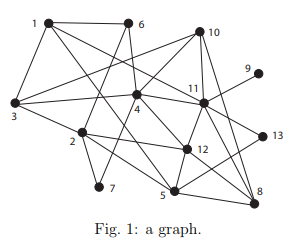
\includegraphics[scale=0.7]{graph}
\end{center}
\begin{solution}[2in]
If a vertex has less than n neighbours (where n is the number of colours to be tested), then it can be removed from the graph, and if the remaining subgraph can be coloured with n colours then the larger graph can also be coloured using n colours.\\
\\
By repeatedly performing this on figure 1 you get to the point where all the nodes have been removed, this can trivially be 4 coloured
\end{solution}

\question[2]What do we mean by a brute-force algorithm to decide whether a graph
can be coloured with 4 colours?
\begin{solution}[2in]
	An algorithm that will try all possible 4 colourings and see if it is legal or not
\end{solution}

\question[3]Suppose that we are given two lists of symbols (possibly of different
lengths). Explain how we order these two lists according to the lexicographic
ordering
\begin{solution}[2in]
	\begin{itemize}
		\item We compare the two lists by working down the lists entry bu entry until two corresponding entries differ
		\item The list with the least entry is determined to be the least of the two lists
		\item If we never find two different corresponding entries but run out of one of the lists then this shortest list is the least list
	\end{itemize}
\end{solution}

\question[5]Give a precise definition of a search problem and of a solution of a
search problem.
\begin{solution}[2in]
	A search problem S consists of:
	\begin{itemize}
		\item A set of instances I
		\item A set of solutions J
		\item A binary search relation $R\subseteq I\times J$
	\end{itemize}
	In order to solve a search problem, for any instance $x\in I$ we need to:
	\begin{itemize}
		\item find a solution $y\in J$ such that $(x,y)\in R$ if there is one, or
		\item Answer no if there is no solution $y$ for which $(x,y)\in R$
	\end{itemize}
\end{solution}
\newpage
\question[1]Explain how there is always a decision problem corresponding to any
search problem.
\begin{solution}[2in]
	If you can find a solution to the search problem, the result is yes to the decision problem
\end{solution}

\question[5]Give a precise definition of an optimisation problem and of a solution
of an instance of an optimisation problem.
\begin{solution}[2in]
	An optimisation problem O is defined as follows:
	\begin{itemize}
		\item It consists of a set of instances I
		\item for every instance $x\in I$ there is a set of feasible solutions f(x)
		\item For every instance $x\in I$ and for every feasible solution $y\in f(x)$ there is a value $v(x,y)\in \mathbb{N}=\{0,1,2,...\}$ giving the measure of the feasible solution y for the instance x
		\item There is a goal which is either min or max
	\end{itemize}
	To solve an optimisation problem, given $x\in I$, we need to find a feasible solution of maximum or minimum measure. It may be the case that:
	\begin{itemize}
		\item There are no feasible solutions for an instance
		\item For a maximisation problem, there are feasible solutions of increasingly large measure
	\end{itemize}
\end{solution}

\question[4]What is the Graph 3-Colouring (decision) problem and what is the
Graph Colouring (optimisation) problem? 
\begin{solution}[2in]
	\begin{itemize}
		\item You are given a plane map of regions, each contained within a continuous border
		\item For any pair of regions, either
		\begin{itemize}
			\item They share no part of a border
			\item Exactly one point of a border, when they do not touch
			\item They share a segment of some border, when they do touch
		\end{itemize}
		\item Can you colour the regions of the map with 3 colours so that if any two regions touch they must be coloured differently
	\end{itemize}
\end{solution}
\newpage
\question[3]What is an independent set in a graph? What is the Independent Set
(optimisation) problem?
\begin{solution}[2in]
	\begin{itemize}
		\item An independent set is a set of vertices in a graph, no two of which are adjacent
		\item The independent set problem:
		\begin{itemize}
			\item An independent set U in a graph $G=(V,E)$ is a subset $I\subseteq V$ of verticies so that no vertex in U is joined by an edge to any other vertex of U
			\item A maximum independent set in G is an independent set of the greatest size possible
		\end{itemize}
	\end{itemize}	
\end{solution}

\question[2]What is the difference between a maximum independent set and a
maximal independent set in a graph?
\begin{solution}[2in]
	A maximal independent set that is not contained in any other independent set
\end{solution}

\question[5]Outline a real-world application of finding independent sets in graphs
(you should explain clearly how finding independent sets is related to
solving the real-world problem).
\begin{solution}[2in]
	\begin{itemize}
		\item The sports day problem is the problem of allocating events to slots such that people participating in multiple events will be able to compete in all events.
		\item An independent set would have all athletes able to take part in all competitions
	\end{itemize}	
\end{solution}


\question[10]Outline a greedy algorithm for finding an independent set in a graph.
Does your algorithm solve the Independent Set (optimisation) problem
(optimally)? (If so then you should explain why; if not then you should
provide a counter-example.) Show how your algorithm proceeds on the
graph in Fig. 1.
\begin{solution}[2in]
\begin{itemize}
	\item We chose the vertex $v$ of our graph with the fewest number of neighbours and add it to the independent set I
	\item We remove $v$ (and its incident edges) as well as all neighbours of $v$ (and their incident edges) from our graph and repeat (with our new, smaller graph)
\end{itemize}
\end{solution}
\newpage
\question[8]Give a graph where as to how you implement your greedy algorithm,
above, matters; that is, where when different possible choices for putting
some vertex in your independent set yields independent sets of different
size.
\begin{solution}[2in]
	\begin{center}
		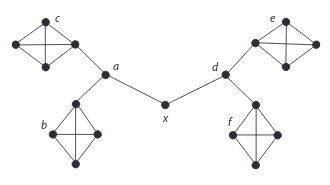
\includegraphics[scale=0.8]{greedy_independent}
	\end{center}
\end{solution}


\question[2]Give two illustrations of principles of Computational Thinking in the
context of problem solving.
\begin{solution}[2in]
	\begin{itemize}
		\item Algorithmic graph theory allows you to analyse graphs, which are used in many of the sciences
		\item The Travelling Salesman Problem can be used for shipping companies to determine optimum distribution routes
	\end{itemize}
\end{solution}
\newpage
\question[10]Outline a greedy algorithm for finding a tour in a given collection of
cities. Does your algorithm solve the Travelling Salesman (optimisation)
problem (optimally)? (If so then you should explain why; if not
then you should provide a counter-example.) Show how your algorithm
proceeds on the following instance of the Travelling Salesman problem
(the city names are in bold and the distances between 2 cities are given
in the table):
\begin{center}
	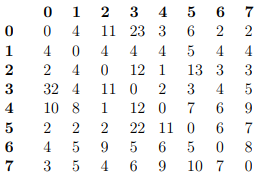
\includegraphics[scale=0.7]{tsptable}
\end{center}
\begin{solution}[2in]
	\begin{itemize}
		\item Start at some node
		\item Iteratively move to the nearest node
		\item Output the tour obtained
	\end{itemize}
One example is made using the paths shown below
	$$\begin{array} { l l l l l l l l l } { } & 
	{ 0 } & { 1 } & { 2 } & { 3 } & { 4 } & { 5 } & { 6 } & { 7 } \\
	 { 0 } & { \textcircled{0} } & { 4 } & { 11 } & { 23 } & { 3 } & { 6 } & { \textcircled{2} } & { 2 } \\
	  { 1 } & { 4 } & { 0 } & { \textcircled{4} } & { 4 } & { 4 } & { 5 } & { 4 } & { 4 } \\ 
	  { 2 } & { 2 } & { 4 } & { 0 } & { 12 } & { \textcircled{1} } & { 13 } & { 3 } & { 3 } \\
	   { 3 } & { \textcircled{32} } & { 4 } & { 11 } & { 0 } & { 2 } & { 3 } & { 4 } & { 5 } \\
	    { 4 } & { 10 } & { 8 } & { 1 } & { 12 } & { 0 } & { \textcircled{7} } & { 6 } & { 9 } \\
	     { 5 } & { 2 } & { 2 } & { 2 } & { 22 } & { 11 } & { 0 } & { 6 } & { \textcircled{7 }} \\ 
	     { 6 } & { 4 } & { \textcircled{5} } & { 9 } & { 5 } & { 6 } & { 5 } & { 0 } & { 8 } \\
	      { 7 } & { 3 } & { 5 } & { 4 } & { \textcircled{6} } & { 9 } & { 10 } & { 7 } & { 0 }
	       \end{array}$$
This gives a tour of 0,6,1,2,4,5,7,3,0 which has length of 58, and follows the above algorithm\\
However in a few places there are multiple choices of where to go, as they all have the same length, so if the below choices are made:
$$\begin{array} { l l l l l l l l l } 
{ } & { 0 } & { 1 } & { 2 } & { 3 } & { 4 } & { 5 } & { 6 } & { 7 } \\
{ 0 } & { 0 } & { 4 } & { 11 } & { 23 } & { 3 } & { 6 } & { \textcircled{2} } & { 2 } \\ 
{ 1 } & { 4 } & { 0 } & { 4 } & { 4 } & { 4 } & { \textcircled{5} } & { 4 } & { 4 } \\ 
{ 2 } & { 2 } & { 4 } & { 0 } & { 12 } & { 1 } & { 13 } & { 3 } & { \textcircled{3} } \\
 { 3 } & { 32 } & { 4 } & { 11 } & { 0 } & { \textcircled{2} } & { 3 } & { 4 } & { 5 } \\
  { 4 } & { 10 } & { 8 } & { \textcircled{1} } & { 12 } & { 0 } & { 7 } & { 6 } & { 9 } \\
   { 5 } & { \textcircled{2} } & { 2 } & { 2 } & { 22 } & { 11 } & { 0 } & { 6 } & { 7 } \\
    { 6 } & { 4 } & { 5 } & { 9 } & { \textcircled{5} } & { 6 } & { 5 } & { 0 } & { 8 } \\
     { 7 } & { 3 } & { \textcircled{5} } & { 4 } & { 6 } & { 9 } & { 10 } & { 7 } & { 0 }
      \end{array}$$
This is following the algorithm as well, but produces the tour of 0,6,3,4,2,7,1,5 which has length 25, so the first time was not optimal. This tour is not necessarily optimal, but given it is smaller than the first attempt then the first attempt cannot be optimal. 
   
\end{solution}




\end{questions}

		
	
	
	
\end{document}